\section{Dataset}

To train and evaluate the vehicle detection pipeline, a custom dataset of real-world 
NYC traffic  was required. Rather than relying on pre-existing generic vehicle 
datasets (ex. Stanford Cars \cite{Krause2013CollectingAL} or BIT-Vehicle\cite{dong_vehicle_2015}), 
this study utilized publicly available traffic camera closed-circuit television 
(CCTV) feeds. This is because the physical camera infrastructure is already installed  
on hundreds of streets across the five boroughs, eliminating the need for new 
equipment and installations. Additionally, images collected from the NYC CCTV 
traffic cameras have a unique resolution and viewing angles, making it difficult 
to generalize vehicles from other datasets to vehicles from NYC CCTV images. 
Furthermore, recent state legislation authorized the New York City Department 
of Transportation (NYC DOT) to quadruple its automated camera network, expanding 
to 600 equipped intersections by the end of 2026 \cite{office_of_the_governor_2024}. 
By tapping into this existing and continually expanding network, 
this methodology ensures that the proposed vehicle detection pipeline can be 
deployed and scaled citywide with zero additional physical infrastructure work.

\subsection{Data Source}

The primary source of images was the 511NY portal, an official service operated 
in conjunction with the New York State Department of Transportation (NYSDOT), 
the New York City Department of Transportation (NYC DOT), and private video 
distribution networks such as Skyline
\cite{NYCDOT_data_feeds} \cite{NYSDOT_c038145_2025} \cite{511ny_about_rideshare}.
The 511NY system provides real-time traffic and transit information, including 
access to hundreds of live traffic cameras deployed across the five boroughs
\cite{NYCDOT_realtime}.

The data can be accessed online through an online GUI or through the 511NY 
Developer REST API. Developers with access to this API can query various 
transportation endpoints, including 
\verb|GetCameras|, \verb|GetEvents|, and \verb|GetMessageSigns| \cite{511ny_api_docs}. 
The \verb|GetCameras| endpoint was primarily queried as it returned metadata for a 
camera's unique ID, exact coordinates (latitude and longitude), the roadway name,
and a URL to fetch the current camera image.

However, querying this endpoint only returned cameras operated by NYSDOT and 
Skyline rather than the complete city network. This limitation exists because 
state and city agencies share data differently. While NYSDOT camera feeds are 
freely accessible through the 511NY API, the New York City Department of 
Transportation (NYC DOT) requires developers to sign a formal data-sharing 
agreement to access its network of over 900 municipal cameras
\cite{NYCDOT_data_feeds} \cite{NYCDOT_realtime_metadata_2010}.
To ensure this research remains easily reproducible without legal barriers, 
the dataset was built exclusively using the unrestricted NYSDOT and Skyline feeds.

\subsection{Collection Protcol and Camera Hardware}

Because querying the global \verb|GetCameras| endpoint only returned a subset of the 
total network, a collection script was developed in Python to save specific, 
known camera images directly. Although the 511NY API allows up to 10 requests per
minute (once every six seconds), and the physical cameras refresh their static 
feeds approximately every 15 seconds, a sampling rate of two minutes was chosen
\cite{511ny_api_docs} \cite{NYCDOT_realtime_subscribers}. 
This was selected to align with New York City's traffic signal cycles, which 
typically range from 45 to 120 seconds depending on local traffic volumes and 
intersection patterns \cite{NYCDOT_traffic_signals}. 
By capturing frames every two minutes, the collection 
protocol inherently acts as a temporal filter, increasing the likelihood that 
consecutive images capture distinct vehicles rather than oversampling the same 
traffic scene.

The physical infrastructure powering these feeds are industrial-grade pan-tilt-zoom
(PTZ) cameras. According to NYSDOT engineering specifications, the standard hardware 
deployed for these remote traffic monitoring tasks includes the Pelco Esprit Model 
ES31PC22-2N, legacy Pelco 9760 units, and Axis Communications Q1614-E models
\cite{NYCDOT_item_2014} \cite{NYCDOT_item_2024}.

\begin{figure}[!htbp]
  \centering

  \begin{subfigure}[c]{0.32\textwidth}
    \centering
    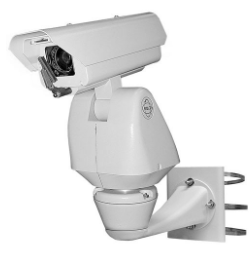
\includegraphics[height=4cm]{figures/dataset/3_2_pelco_esprit_camera.png}
    \caption{Pelco Esprit ES31PC22-2N \cite{bh_photo_video_pelco_2026}.}
  \end{subfigure}
  \hfill
  \begin{subfigure}[c]{0.32\textwidth}
    \centering
    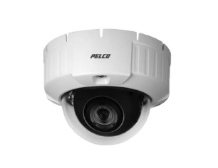
\includegraphics[height=4cm]{figures/dataset/3_2_pelco_9760_camera.png}
    \caption{Pelco 9760 \cite{froehlich5220_pelco_2026}.}
  \end{subfigure}
  \hfill
  \begin{subfigure}[c]{0.32\textwidth}
    \centering
    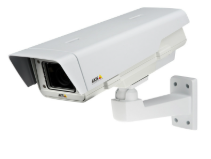
\includegraphics[height=4cm]{figures/dataset/3_2_axis_camera.png}
    \caption{Axis Q1614-E \cite{axis_communications_axis_2026}.}
  \end{subfigure}

  \caption{Example PTZ camera models used in NYSDOT/NYC traffic monitoring infrastructure. Note: camera sizes are not to scale.}
  \label{fig:ptz-cameras}
\end{figure}
